\section{Learning from Data}
Each graphical model consists of two major components - the graph structure, and the potentials given the graph structure. 
\subsection{Graph Structure}
There are two major methods to learn the graph:
\begin{enumerate}
	\item \textbf{Manual:} A domain expert manually designs the graphs. This is popular in applications where we are well-versed with the underlying dependency structure. For example - Quick Medical Reference (QMR) systems for disease-symptoms matching, Kalman Filters, Grid graphs in Computer Vision, Hidden Markov Models (HMM) in speech recognition/information extraction.
	\item \textbf{Learning from Examples:} It can be shown that recovering the graph structure is NP hard. Usually learning methods are branch and bound search problems, which are particularly useful in dynamic situations.
\end{enumerate}
\subsection{Parameters in Potentials}
As before, there are the two same methods for learning:
\begin{enumerate}
	\item \textbf{Manual:} Done by a domain expert usually for infrequently constructured graphs (QMR systems), or where the potentials are a trivial function of the attributes of the connected graphs (grid graphs). This is a relevant method for Bayesian Networks, as potentials correspond to conditional probabilities. Thus in data-starved regions, with priors we can use Bayesian Networks.
	\item \textbf{Learning from Examples:} A popular method where humans cannot make objective assignments. Two major subdomains are table potentials, where each entry is a parameter (HMMs), and potentials with shared parameters and data attributed (CRFs).
\end{enumerate}
Given a sample of data $\mathcal D$ generated from a distribution $P$, being represented by a known graphical model $G$, our aim is to learn the potentials. There can be many scenarios to consider -
\begin{enumerate}
	\item \textbf{Variables:}
	\begin{enumerate}
		\item In each training instance, we have observed all the variables $\mathcal{X}$. Such a setting is called fully supervised setting.
		\item In each training instance, we have observed a subset of variables $\mathfrak{X} \subset \mathcal{X}$. Such a setting is called partially observed setting.
	\end{enumerate}
	\item \textbf{Potentials:}
	\item In BNs, we don't have a log-partition function $\log Z$, and thus in most cases, we'd be able to find closed form solutions for potentials.
	\item In UGMs, $\log Z$ causes a lot of trouble. Since potentials are attached to arbitrary overlapping subset of variables, we require gradient descent kind of iterative algorithms.
\end{enumerate}
Representation of potentials as parameters includes - 
\begin{enumerate}
	\item \textbf{Generative:} 
	$P(\mathbf x) = P(x_1, \cdots, x_n)$ is represented as our $G$. The training samples are $\mathcal{D} = \{\mathbf{x}^1, \cdots, \mathbf{x}^N\}$ where
	$\mathbf{x}^i = \{x_1^i, x_2^i, \cdots, x_n^i\}$, and we finally learn the potentials $\psi_C(\mathbf x_C)$.
	\item \textbf{Conditional:}
	We work with $P(\mathbf{y|x}) = P(y_1, \cdots, y_n|\mathbf x)$ represented by our $G$ over $\mathbf{y}$ variables. Our training instances in this case would be 2-tuples $\mathcal{D} = \{(\mathbf{x}^1, \mathbf{y}^1), \cdots, (\mathbf{x}^N), \mathbf{y}^N\}$ and we learn the potentials $\psi_C(\mathbf{y}_C, \mathbf x)$.
\end{enumerate}
\subsection{Learning under Conditional Representation}
We now focus on the conditional representation of potentials, and provide a general framework for parameter learning. \\
Consider the conditional distribution $\Prob(\mathbf y|\mathbf x, \theta)$, potentials are function of $\mathbf{x}$, and we want to learn $\theta$. Say $\mathbf y = y_1, \cdots, y_n$ forms a graphical model $G$. \\
Say $G$ is undirected, then
\begin{equation}
\begin{split}
	\Prob(y_1, \cdots, y_n | \mathbf x, \theta) &= \dfrac{\prod_C \psi_C(\mathbf y_C, \mathbf x, \theta)}{Z_\theta(\mathbf x)} \\&= \dfrac{1}{Z_\theta(\mathbf x)}\exp\bigg(\sum_C F_\theta(\mathbf y_C, C, \mathbf x)\bigg)
\end{split}
\end{equation} 
where $F_\theta(\mathbf y_C, C, \mathbf x) = \log \psi_C (\mathbf y_C, \mathbf x, \theta)$, $Z_\theta(\mathbf x) = \sum_{\mathbf y'} \exp\bigg(\sum_C F_\theta(\mathbf y'_C, C, \mathbf x)\bigg)$. \\
Now, we can think of $F_\theta(\mathbf y_C, C, \mathbf x)$ in many ways
\begin{enumerate}
	\item \textbf{Log-linear model} over features defined by the user (eg. in CRFs, Maxent models). Say we gave $K$ features, and each feature is represented as $f_k(\mathbf y_C, C, \mathbf x)$. Thus, 
	\begin{equation}
		F_\theta(\mathbf y_C, C, \mathbf x) = \sum_{k=1}^K \theta_k f_k(\mathbf y_C, C, \mathbf x) 
	\end{equation}
   \item \textbf{Neural Network} which takes in $\mathbf y_C, C, \mathbf x$ and transforms them non-linearly into $\mathcal{Y} \in \R$, and $\theta$ are the parameters of the neural network.
\end{enumerate}
\begin{exmp}[Named Entity Recognition]
Consider the task of NER, where $y_i$ can take 3 values, and the structure is represented as a chain graph. Thus essentially, the user enforces that only adjacent words in the sentence affect the labels taken. Since we have a chain graph, we take the cliques as edges, and we take our templatized functions as $\mathbf{f}(y_i, y_{i-1}, i, \mathbf{x})$, where $C=i$ is a short hand for $C = (i-1, i)$. Defining the features $f_i(y_i, y_{i-1}, i, \mathbf{x})$. We can manually write heuristics, or in something like BERT, we can have $\mathbf{f}(y_i, y_{i-1}, i, \mathbf x) = \mathbf e_i \in \R^K$ where $e_i$ is the embedding generated by BERT.
\end{exmp}
Now, for training, we have been given $N$ input pairs represented by $\mathcal{D} = \{(\mathbf x^1, \mathbf y^1), \cdots, (\mathbf x^N, \mathbf y^N)\}$, and the form of $F_\theta$. We learn $\theta$ through maximum likelihood, i.e
\begin{equation}
	\begin{split}
	\max_{\theta} LL(\theta, \mathcal D) &= \max_\theta \sum_{i=1}^N \log\Prob(\mathbf{y}^i|\mathbf{x}^i, \theta)
	\end{split}
\end{equation}
We can write
\begin{equation}
\begin{split}
	LL(\theta, \mathcal{D}) &= \sum_{i=1}^N \log\Prob(\mathbf{y}^i|\mathbf{x}^i, \theta) \\
	&= \sum_{i=1}^N \log\bigg(\dfrac{1}{Z_\theta(\mathbf x^i)} \exp\Big(\sum_C F_\theta(\mathbf y^i_C, C, \mathbf x^i)\Big)\bigg) \\
	&= \sum_{i=1}^N \Bigg[\sum_C F_\theta(\mathbf y^i_C, C, \mathbf x^i) - \log Z_\theta(\mathbf x^i) \Bigg]
\end{split}
\end{equation}
Note that computing $F_\theta$ is not difficult, but to calculate $Z_\theta$ for each $i$ requires invoking an inference algorithm. \\
For training, we can use gradient descent. For now, let us assume a log-linear model as $F_\theta(\mathbf y_C^i, C, \mathbf x) = \theta\cdot \mathbf f(\mathbf x^i, \mathbf y^i_C, C)$, and denote $\mathbf f(\mathbf x^i, \mathbf y^i) = \sum_C\mathbf f(\mathbf x^i, \mathbf y^i_C, C)$. Thus,
\begin{equation}
LL(\theta) = \sum_{i} \Big(\theta\cdot\mathbf f(\mathbf x^i, \mathbf y^i) - \log Z_\theta(\mathbf x^i) \Big)
\end{equation}
We can add a regularizer to prevent over-fitting. Thus, our objective becomes
\begin{equation}
	\max_{\theta} \sum_i \Big(\theta\cdot\mathbf f(\mathbf x^i, \mathbf y^i) - \log Z_\theta(\mathbf x^i) \Big) - \dfrac{\|\theta\|^2}{C}
\end{equation}
The objective function is concave in $\theta$, and thus we can reach the globally optimal value of $\theta$ using gradient descent. The gradient of the objective $L(\theta)$ is 
\begin{equation}
\begin{split}
	\nabla L(\theta) &=  \sum_i \bigg(\theta\cdot\mathbf f(\mathbf x^i, \mathbf y^i) - \dfrac{\sum_{\mathbf y'} \mathbf f(\mathbf y', \mathbf x^i) \exp(\theta \cdot \mathbf f(\mathbf x^i, \mathbf y^i))}{Z_\theta(\mathbf x^i)}\bigg) - \dfrac{2\theta}{C} \\
	&= \sum_i \Big(\theta\cdot\mathbf f(\mathbf x^i, \mathbf y^i) - \sum_{\mathbf y'} \mathbf f(\mathbf x^i, \mathbf y^i)\Prob(\mathbf y'|\theta, \mathbf x^i)\Big) - \dfrac{2\theta}{C} \\
	&= \sum_i \bigg(\theta\cdot\mathbf f(\mathbf x^i, \mathbf y^i) - \mathbb{E}_{\Prob(\mathbf y'| \theta, \mathbf x')} \mathbf f(\mathbf x^i, \mathbf y^i)\Big) - \dfrac{2\theta}{C}
\end{split} 
\end{equation}
where 
\begin{equation}
\begin{split}
	\mathbb{E}_{\Prob(\mathbf y'| \theta, \mathbf x')} f_k(\mathbf x^i, \mathbf y') &= \sum_{\mathbf y'}  f_k(\mathbf x^i, \mathbf y')\Prob(\mathbf y'|\theta, \mathbf x^i) \\
	&= \sum_{\mathbf y'} \sum_C f_k(\mathbf x^i, \mathbf y'_C, C)\Prob(\mathbf y'|\theta, \mathbf x^i) \\
	&= \sum_C \sum_{\mathbf y_C'} f_k (\mathbf x^i, \mathbf y_C', C)\Prob(\mathbf y_C'|\theta, \mathbf x^i)
\end{split}
\end{equation}
\begin{exmp}\label{exmp:i-1}
Consider an undirected graphical model on 3 binary variables $\{y_1, y_2, y_3\}$ represented as $\mathbf y$, and are forming a chain. We define two features for the model as
\[
\begin{split}
	f_1(\mathbf x, y_j, j) &= x_jy_j \qquad \text{where $x_j$ is the intensity of pixel $j$} \\
	f_2(\mathbf x, (y_k, y_j), (k,j)) &= [\![ y_k \neq y_j ]\!] \qquad \text{where $[\![\alpha]\!] = 1$ if $\alpha=$true}
\end{split}
\]
Consider the initial parameters as $\theta = [\theta_1, \theta_2] = [3,-2]$, and consider $\mathbf x^1 = [0.1, 0.7, 0.3]$ and $\mathbf y^1 = [1, 1, 0]$. \\
\begin{itemize}
	\item[$\diamond$] The log-node potentials $F_\theta(y_j, C=j, \mathbf x)$ are given as $$y_j = \theta \cdot \mathbf f(\mathbf x, y_j, j) = \theta_1 x_j y_j$$
	For $y_1$, we have the value as $[0, 0.3]$, $y_2$ will have the value $[0, 2.1]$ and $y_3$ will have $[0, 0.09]$.
	\item[$\diamond$] The log-edge potentials $F_\theta((y_1, y_2), C=(1,2), \mathbf x)$ are given as
	\[\theta_2f_2(\mathbf x, (y_1, y_2), (1,2))\]
	For $(1,2)$ we have the value as $[0, -2, 0, -2]$ corresponding to $y_1y_2 = \{00, 01, 10, 11\}$ (can consider it to be a matrix for ease of understanding). Since our edge potentials don't depend on $x$, $F_\theta((y_2,y_3), C=(2,3), \mathbf x) = [0, -2, -2, 0]$. 
\end{itemize}
\end{exmp}
\begin{exmp}
Consider parameter learning for $\mathbf y = \{y_1, \cdots, y_6\}$, where $y_j = \pm 1$. Let us define 8 features for the variables as
\begin{align*}
f_1 (y_j, y_{j+1}) &= [\![ y_j + y_{j+1} > 1 ]\!], \quad 1 \leq j \leq 5 \\
f_2(y_1, y_3) &= -2y_1y_3 \\
f_3(y_2, y_3) &= y_2y_3 \\
f_4(y_3, y_4) &= y_3y_4 \\
f_5(y_2, y_4) &= [\![y_2y_4<0]\!] \\
f_6(y_4, y_5) &= 2y_4y_5 \\
f_7(y_3,y_5) &= -y_3y_5 \\
f_8(y_5,y_6) &= [\![y_5+y_6>0]\!] 
\end{align*}
Consider 
\[\mathbf{f(y)} = [f_1, \cdots, f_8] \text{ and } \theta=[1\; 1\; 1 \;2 \;2 \;1 \;-1 \;1]^\top\]
\begin{marginfigure}
	\centering
	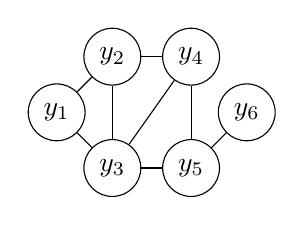
\begin{tikzpicture}[main/.style = {draw, circle}] 
		\node[main] (1) {$y_1$}; 
		\node[main] (2) [above right of=1] {$y_2$}; 
		\node[main] (3) [below right of=1] {$y_3$}; 
		\node[main] (4) [right of=2] {$y_4$}; 
		\node[main] (5) [right of=3] {$y_5$}; 
		\node[main] (6) [below right of=4] {$y_6$}; 
		\draw[-] (1) -- (2);
		\draw[-] (1) -- (3);
		\draw[-] (2) -- (3);
		\draw[-] (2) -- (4);
		\draw[-] (3) -- (4);
		\draw[-] (3) -- (5);
		\draw[-] (4) -- (5);
		\draw[-] (5) -- (6);
	\end{tikzpicture}
	\caption{UGM for example}
	\label{fig:l-exmp-6}		
\end{marginfigure}
The underlying graphical model is given in Figure \ref{fig:l-exmp-6}
For the above graph, we can draw the junction tree to find 
\[Z = \sum_{\mathbf y} \exp\Big(\theta^\top \mathbf{f(x,y)}\Big)\]
For clique $C$, we have $\psi_C(\mathbf y_C) = \exp\Big(\theta \cdot \mathbf{f}_C(\mathbf x,\mathbf y_C)\Big)$. 
\begin{marginfigure}
	\centering
	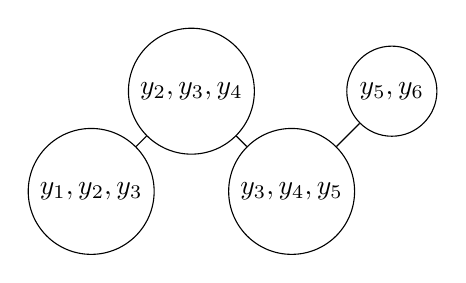
\begin{tikzpicture}[main/.style = {draw, circle}, node distance=1.8cm] 
		\node[main] (123)  {$y_1,y_2,y_3$}; 
		\node[main] (234) [above right of=123]{$y_2, y_3,y_4$}; 
		\node[main] (345) [below right of=234]{$ y_3,y_4,y_5$}; 
		\node[main] (56) [above right of=345] {$y_5, y_6$}; 
		\draw[-] (123) -- (234);
		\draw[-] (234) -- (345);
		\draw[-] (345) -- (56);
	\end{tikzpicture}
	\caption{JT for above UGM}
	\label{fig:l-exmp-6-jt}		
\end{marginfigure}
The junction tree for the above graph is given in Figure \ref{fig:l-exmp-6-jt}. Say from left to right in the JT, we call the cliques $\mathscr C_1$ to $\mathscr C_4$. For $\mathscr C_2$, the log-potential will be $2 \cdot f_5(y_2, y_4) + 1 \cdot f_1(y_3, y_4) + 2\cdot f_4(y_3, y_4)$. We can easily find for others too.
\end{exmp}
Now, coming back to the expectation, we need to compute \\ $\mathbb{E}_{\Prob(\mathbf y|\theta^\top, \mathbf x^i)}f_k(\mathbf x^i, \mathbf y)$. To do this, we can proceed as follows:
\begin{enumerate}
	\item Represent the probability $\Prob(\mathbf y|\theta^\top, \mathbf x^i)$ as UGM where nodes are $y_1, \cdots y_n$ and the potential $\psi_C(\mathbf y_C, \mathbf x, \theta)$ for clique $C$ is $\exp\big(\theta^\top \cdot \mathbf f(\mathbf x^i, \mathbf y_C^i, C)\big)$.
	\item Run a sum-product inference algorithm on the above UGM and compute for each $C$, $\mathbf y_C$ the marginal probability $\mu(\mathbf y_C, C, \mathbf x^i)$.
	\item Using these nodes, compute 
	\[\mathbb{E}_{\Prob(\mathbf y|\theta^\top, \mathbf x^i)}f_k(\mathbf x^i, \mathbf y) = \sum_C\sum_\mathbf{y_C} \mu(\mathbf y_C, C, \mathbf x^i)f_k(\mathbf x^i, C, \mathbf y_C)\]
\end{enumerate}
Having done this, we continue Example \ref{exmp:i-1}. We can calculate marginals $\mu(y_j, j)$ and $\mu(y_k, y_j, (k,j))$, and write
\begin{align*}
\mathbb{E}[f_1(\mathbf x^1, \mathbf y)] &= \sum_j \sum_{y_j'} \mu_j(y_j', j)x_jy_j' =\sum_j y_jx_j \mu_j(1,j) \\&= 0.1\mu(1,1) + 0.7 \mu(1,2) + 0.3\mu(1,3) \\
\mathbb{E}[f_2(\mathbf x^2, \mathbf y)] &= \sum_C \sum_{y_C'} \mu_j(y_C', C)f_2(y_C', C, x)\\&= \mu(1,0,(1,2)) + \mu(0,1, (1,2)) + \mu(1,0,(2,3)) + \mu(0,1, (2,3))
\end{align*}
Now, value of 
\begin{align*}
f_1(\mathbf x^1, \mathbf y^1) &= \sum_C f_1(\mathbf x^1, \mathbf y^1_C, C) = \sum_{j=1}^3 f_1(\mathbf x^1, y^1_j, j) = \sum_{j=1}^3 x_jy_j\\
&= 0.1 \times 1 + 0.7 \times 1 + 0.3 \times 0 = 0.8 \\
f_2(\mathbf x^1, \mathbf y^1) &= [\![y_1^1 \neq y_2^1]\!] + [\![y_2^1 \neq y_3^1]\!] = 1
\end{align*}
Thus we can write the gradients for each parameter as
\begin{align*}
\nabla L(\theta_1) &= 0.8 - \mathbb{E}(f_1(\mathbf x^1, \mathbf y)) - 2\cdot\dfrac{3}{C} \\
\nabla L(\theta_2)&=  1 - \mathbb{E}(f_2(\mathbf x^1, \mathbf y)) + 2\cdot\dfrac{2}{C} 
\end{align*}
\subsection{Training Algorithm}
\begin{algorithm}[H]\label{alg:l-train}
	\DontPrintSemicolon
	\textbf{Input:} $\mathcal{D} = \{(\mathbf x^i, \mathbf y^i)\}_{i=1}^N$, $\mathbf f: f_1, \cdots, f_K$\;
	\textbf{Output:} $\theta = \argmax \sum_{i=1}^N (\theta \cdot \mathbf f(\mathbf x^i, \mathbf y^i) - \log Z_\theta (\mathbf x^i)) - \frac{\|\theta\|^2}{C}$\;
	\textbf{Initialize:} $\theta^0 = \mathbf 0$\;
	\For{$t=1$ to $T$}{
		\For{$i=1$ to $N$}{
			$g_{k,i} = f_k(\mathbf x^i, \mathbf y^i) - \mathbb{E}_{\Prob(\mathbf y'|\theta^\top, \mathbf x^i)}f_k(\mathbf x^i, \mathbf y')$ for $k=1,\cdots,K$\;
		}
	$g_k = \sum_i g_{k,i}$ for $k=1, \cdots, K$\;
	$\theta_k^t = \theta_k^{t-1} + \gamma_t(g_k - 2\frac{\theta_k^{t-1}}{C})$\;
	\textbf{Exit:} if $\|\mathbf g\| \approx 0$\;
	}
	\caption{Training Algorithm for Parameter Learning}
\end{algorithm}
The running time for Algorithm \ref{alg:l-train} in case of chain graph is $\mathcal{O}(INn(m^2+K))$ where $I$ is the total number of iterations. But in general, for a graph with tree-width of $w$, the running time has $m^{w+1}$ instead of $m^2$. \\
The above algorithm is a generalized framework, and we can see its use in Bayesian Networks now.
\subsection{Local Conditional Probability for Bayesian Networks} 
\noindent For a Bayesian Network
\begin{equation}
	\begin{split}
	\Prob(y_1, \cdots, y_n|\mathbf x, \theta) &= \prod_j \Prob(y_j|\mathbf y_{\text{Pa}(j)}, \mathbf x, \theta) \\
	&= \prod_j \dfrac{\exp\big(F_\theta(\mathbf{y}_{\text{Pa}(j)}, y_j, j, \mathbf x)\big)}{\sum_{y'_j=1}^m \exp\big(F_\theta(\mathbf{y}_{\text{Pa}(j)}, y'_j, j, \mathbf x\big)}
	\end{split}
\end{equation}
The potentials above are locally normalized. Now, we can write the likelihood as
\begin{equation}
	\begin{split}
LL(\theta, \mathcal D) &= \sum_{i=1}^N \log \Prob(\mathbf y^i|\mathbf x^i, \theta) \\
&= \sum_{i=1}^N \log\bigg(\prod_j \Prob(y^i_j|\mathbf y^i_{\text{Pa}(j)}, \mathbf x^i, \theta)\bigg) \\
&=\sum_{i}\sum_j \log \Prob(y^i_j|\mathbf y^i_{\text{Pa}(j)}, \mathbf x^i, \theta) \\
&= \sum_i\sum_j F_\theta(\mathbf{y}^i_{\text{Pa}(j)}, y^i_j, j, \mathbf x^i) - \log\sum_{y'=1}^m \exp\big(F_\theta(\mathbf{y}^i_{\text{Pa}(j)}, y'_j, j, \mathbf x^i\big)
	\end{split}
\end{equation}
We can notice that we are essentially doing a softmax over $F_\theta(\cdot)$, and thus we are doing a normal classification task.
\subsection{Table Potentials in Feature Framework}
Consider a generative model (i.e $\mathbf x^i$ does not exist) - such as an Hidden Markov Model. 
\begin{itemize}
	\item[$\diamond$] $F_{\theta}(\mathbf y_{\text{Pa}(j)}^i, y_j^i, j) = \log P(y_j^i, \mathbf y_{\text{Pa}(j)}^i)$, and the normalizer vanishes.
	\item[$\diamond$] $\Prob(y_j|\mathbf y_{\text{Pa}(j)})$ is a table of real values denoting the probability of each value of $x_j$ corresponding to each combination of values of the parents ($\theta^j$).
	\item If each variable takes $m$ values, and has $k$ parents, then each $\Prob(y_j|\mathbf y_{\text{Pa}(j)})$ will require $m^{k+1}$ parameters in $\theta^j$.
	\begin{equation}
	\theta^j_{vu_1, \cdots, u_k} = \Prob(y_j = v|\mathbf{y}_{\text{Pa}(j)} = [u_1, \cdots, u_k])
	\end{equation}
\end{itemize}
\begin{marginfigure}
	\centering
	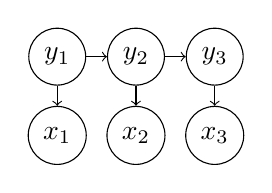
\begin{tikzpicture}[main/.style = {draw, circle}] 
		\node[main] (y1)  {$y_1$}; 
		\node[main] (y2) [right of=y1] {$y_2$};
		\node[main] (y3) [right of=y2] {$y_3$};
		\node[main] (x1) [below of=y1] {$x_1$};
		\node[main] (x2) [below of=y2] {$x_2$};
		\node[main] (x3) [below of=y3] {$x_3$};
		\draw[->] (y1) -- (x1);
		\draw[->] (y1) -- (y2);
		\draw[->] (y2) -- (x2);
		\draw[->] (y2) -- (y3);
		\draw[->] (y3) -- (x3);
	\end{tikzpicture}
	\caption{Sample HMM}
	\label{fig:l-exmp-2}	
\end{marginfigure}
\begin{exmp}[HMM Parameter Learning]
Consider the HMM shown in Figure \ref{fig:l-exmp-2}. Say $y_j \in \{1,2,3\}$ and $x_j \in \{A,B,C,D\}$.
\begin{table}[h]
	\centering
	\begin{tabular}{|c|c|c|c|}
		\hline
		$(y_1, x_1)$ & $(y_2, x_2)$ & $(y_3, x_3)$ & $(y_4,x_4)$ \\ \hline
		1, A         & 1, B         & 2, A         & 3, C        \\ \hline
		2, B         & 1, A         & 3, A         & 3, D        \\ \hline
		1, B         & 1, B         & 2, C         & 3, D        \\ \hline
	\end{tabular}
	\caption{}
	\label{tab:l-exmp-2}
\end{table}
The above table contains the values for $\mathcal {D} = (N=3, n=4)$. We need to calculate the probability of variable given its parent. Since $y_1$ has no parent, we can write
\begin{equation*}
	P(y_1) = 
	\centering
	\begin{tabular}{|c|c|c|}
		\hline
		1             & 2             & 3 \\ \hline
		$\frac{2}{3}$ & $\frac{1}{3}$ & 0 \\ \hline
	\end{tabular}
\end{equation*}
The values from left to right denote $\theta_1^1, \theta_2^1, \theta_3^1$. For $y_2$ we need to find $\theta^2_{v:u} = P(y_2=v|y_1=u)$ and this will have 9 values. 
\begin{equation*}
	P(y|y') = 
	\centering
	\begin{tabular}{|c|c|c|c|}
		\hline
		& $y=1$         & $y=2$         & $y=3$         \\ \hline
		1 & $\frac{2}{5}$ & $\frac{2}{5}$ & $\frac{1}{5}$ \\ \hline
		2 & $\frac{1}{3}$ & 0             & $\frac{2}{3}$ \\ \hline
		3 & 0             & 0             & 1             \\ \hline
	\end{tabular}
\end{equation*}
Now, to find $\theta^{x_1}_{u:v} = P(x_1=u, y_1=v)$, we will have 12 values. 
\end{exmp}
For the above, we can notice that
\begin{align*}
	LL(\theta, \mathcal D) &= \max_\theta \sum_i \sum_j \log P(y_j^i|\mathbf{y}^j_{\text{Pa}(j)}) \\
	&= \max_\theta \sum_i \sum_j \log \theta^j_{y_j\mathbf{y}_{\text{Pa}(j)}} \quad \text{s.t } \sum_v \theta^J_{vu_1, \cdots, u_k} = 1 \; \forall \; j, u_1, \cdots, u_k \\
	&= \max_\theta \sum_i \sum_j \log \theta^j_{y_j\mathbf{y}_{\text{Pa}(j)}} - \sum_j \sum_{u_1, \cdots, u_k} \lambda^j_{u_1, \cdots, u_k} \bigg(\sum_v \theta^j_{vu_1, \cdots, u_k} - 1 \bigg)
\end{align*}
Using gradient descent, we can get that
\begin{equation}
	\theta^j_{vu_1, \cdots, u_k} = \dfrac{\sum_{i=1}^N [\![y_j^i = v, \mathbf{y}_{\text{Pa}(j)} = u_1, \cdots, u_k]\!]}{\sum_{i=1}^N[\![\mathbf{y}_{\text{Pa}(j)} = u_1, \cdots, u_k]\!] }
\end{equation}
Going back to the previous example, we can write for $P(y_1)$, the variables 
\[\theta_1^1 = \dfrac{\sum_{i=1}^3 [\![y_1^i=1]\!]}{\sum_{i=1}^3 [\![1]\!]} = \dfrac{2}{3}\] 
Now for the second table, look at the first entry $2/5$. We find all those values, where the next variable is $1$, given the  previous variable is $1$. This occurs two times, and $1$ occurs 5 times, giving the value 2/5. Note that this has occurred due to parameter sharing, i.e $\theta^{y_2}_{v:u} = \theta^{y_3}_{v:u} = \theta^{y_4}_{v:u}$. This allows us to use variable length sentences. 
\subsection{Neural Translation Models}
Say $X$ is a sentence in English having $m$ tokens, an $Y$ is a sentence in Hindi having $n$ tokens. We want to create $P(Y|X)$. Say our Hindi dictionary has size $30000$, then the number of sentences of length $n$ you can create is $(30000)^n$. A simpler method would be 
\begin{equation}
	P(Y|X) = \prod_{j=1}^n P(y_j|y_1, \cdots, y_{j-1}, X)
\end{equation}
The above gives a complete factorization. To learn the potentials, we would have to come up with a way to make the given set capable of handling variable length sentences. We can parameterize using a neural network that can handle variable length inputs such as RNNs and Transformers. For an RNN, we have $s_t$ as an embedding for $y_1, \cdots, y_{j-1}$ and is computed recursively.
\begin{align*}
	s_0 &\longleftarrow \text{ initial state} \\
	s_t &\longleftarrow \text{ LSTMcell}(\theta, s_{t-1}, y_{t-1}) \\
	v_t &\longleftarrow \text{ embedding of } X
\end{align*}
\[P(y_j | y_1, \cdots, y_{j-1}, X) \equiv Softmax(\{y_j\}, NN_\theta [s_t, v_t])\]
Thus, we get a standard classification problem, i.e given a $X$, find the $Y$ for which $P(Y|X)$ is maximized. The is intractable for chain graph, and thus in practice greedy inference algorithms such as Beam Search are used.
\subsection{Learning with Hidden Variables}
If we suppose only a subset of variables, how do we learn the parameters of the graphical model?
\begin{marginfigure}
	\centering
	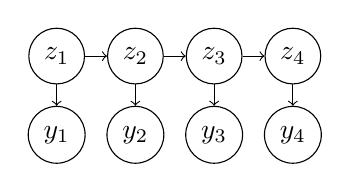
\begin{tikzpicture}[main/.style = {draw, circle}] 
		\node[main] (z1)  {$z_1$}; 
		\node[main] (z2) [right of=z1] {$z_2$};
		\node[main] (z3) [right of=z2] {$z_3$};
		\node[main] (z4) [right of=z3] {$z_4$};
		\node[main] (y1) [below of=z1] {$y_1$};
		\node[main] (y2) [below of=z2] {$y_2$};
		\node[main] (y3) [below of=z3] {$y_3$};
		\node[main] (y4) [below of=z4] {$y_4$};
		\draw[->] (z1) -- (y1);
		\draw[->] (z1) -- (z2);
		\draw[->] (z2) -- (y2);
		\draw[->] (z2) -- (z3);
		\draw[->] (z3) -- (y3);
		\draw[->] (z3) -- (z4);
		\draw[->] (z4) -- (y4);
	\end{tikzpicture}
	\caption{Sample HMM}
	\label{fig:l-exmp-4}	
\end{marginfigure}
Say we have the HMM shown in Figure \ref{fig:l-exmp-4}. Note that we have changed the notation from $x\to y$ and $y\to z$, since $x$ is not a random variable for now. In CRF, we try to learn $P(Y|X)$ with $\mathcal{D} = \{\mathbf x^i, \mathbf y^i\}$, where all variables $y_1^i, \cdots, y_n^i$ are present in the dataset, but here in addition some variables $z_1^i, \cdots z_m^i$ are not present in $\mathcal D$. \\
If we denote $\theta$ as the parameters of the graphical model, then
\begin{equation}
	P_{\theta, G}(y_1, \cdots y_n, z_1, \cdots, z_m|\mathbf x) = \dfrac{1}{Z_{\theta(\mathbf x)}}\exp\Big(\sum_C F_\theta(\mathbf y_C, \mathbf z_C, \mathbf x)\Big)
\end{equation}
where $C$ is the set of cliques in the graph. Suppose $\mathcal D = \{(\mathbf x^i, \mathbf y^i): i=1,\cdots,N\}$ is our dataset, we want to find
\begin{equation}
\begin{split}
	\theta^{ML} &= \argmax_\theta \sum_{i=1}^N \log P_\theta(\mathbf y^i|\mathbf x^i) \\
	&= \argmax_\theta \sum_{i=1}^N \log\bigg( \sum_{\mathbf z} P_{\theta, G}(\mathbf y^i, \mathbf z|\mathbf x^i)\bigg)
\end{split}
\end{equation}
The sum over $\mathbf z$ makes the optimization difficult (because the space of values is large) and thus we want to approximate this, and for this we use a variational approach. \\
In the variational approach, we introduce auxiliary variables and write
\begin{equation}
\begin{split}
&\max_\theta \sum_{i=1}^N \log \sum_{\mathbf z:z_1, \cdots z_m}P(\mathbf y^i, \mathbf z | \theta, \mathbf x^i) \\
&\equiv \max_\theta\sum_{i=1}^N \max_{q_{i,\mathbf z}:\sum_{\mathbf z} q_{i, \mathbf z} = 1} \sum_{\mathbf z} q_{i, \mathbf z} \log P(\mathbf y^i, \mathbf z | \theta, \mathbf x^i) - \sum_{\mathbf z} q_{i, \mathbf z} \log q_{i, \mathbf z}
\end{split}
\end{equation}
This rewriting makes us avoid the summation within the log, and we have two maximization problems - over $\theta$ and all $q$ variables. The inner one can be solved in a closed form for fix $\theta$, and the outer one can be solved like a maximum likelihood problem without hidden variables. We now prove the above result. \\
\begin{proof}
We will show that
\begin{equation}
\begin{split}
\log\sum_{z=1}^k g(y,z) &= \max_{q_1, \cdots, q_k} \sum_{z=1}^k q_z\log g(y,z) - \sum_z q_z\log q_z \\
&s.t. \; \sum_{z=1}^k q_z = 1 \text{ and } q_z \geq 0
\end{split}
\end{equation}
where the variables $q_1$ to $q_k$ are auxiliary, and
\begin{equation}
	Q(q, g) \triangleq \sum_{z=1}^k q_z \log g(y,z) - \sum_z q_z \log q_z
\end{equation}
We use the Lagrangian multipliers method to do so. \\
Let $L(Q,\lambda) = Q(q, g) + \lambda(\sum_z q_z - 1)$. Then we can write
\begin{align*}
\dfrac{\partial L(Q, \lambda)}{\partial q_j} &= \log g(y, j) - \log q_j - 1 + \lambda = 0 \\
&\implies q^*_j \equiv \alpha g(y,j) \\
\sum_z q_z = 1 &: q_j^* = \dfrac{g(y,j)}{\sum_z g(y,z)}
\end{align*}
If we put this value of $q^*$ in the original equation, we get the expression to be equal to $\log\sum_{z=1}^k g(y,z)$ and get the required result. Note that for all other $q$, we have
\[\log\sum_{z=1}^k g(y,z) \geq \sum_{z=1}^k q_z\log g(y,z) - \sum_z q_z\log q_z\]
\end{proof}